\section{Theorie}
\label{sec:Theorie}
Brückenschaltungen werden in der Messtechnik eingesetzt, da mit ihnen die Auflösung
der Messung erhöht werden kann.
In Abbildung \ref{fig:Brueckenschaltung} ist das Bild einer prinzipiellen Brückenschaltung zu sehen.
Die Potentialdifferenz $U$ wird zwischen den Punkten A und B gemessen. Aus der
Knotenregel ergibt sich, dass die Summe der Ströme an einer Verzweigung $0$ ist.


\begin{figure}
  \centering
  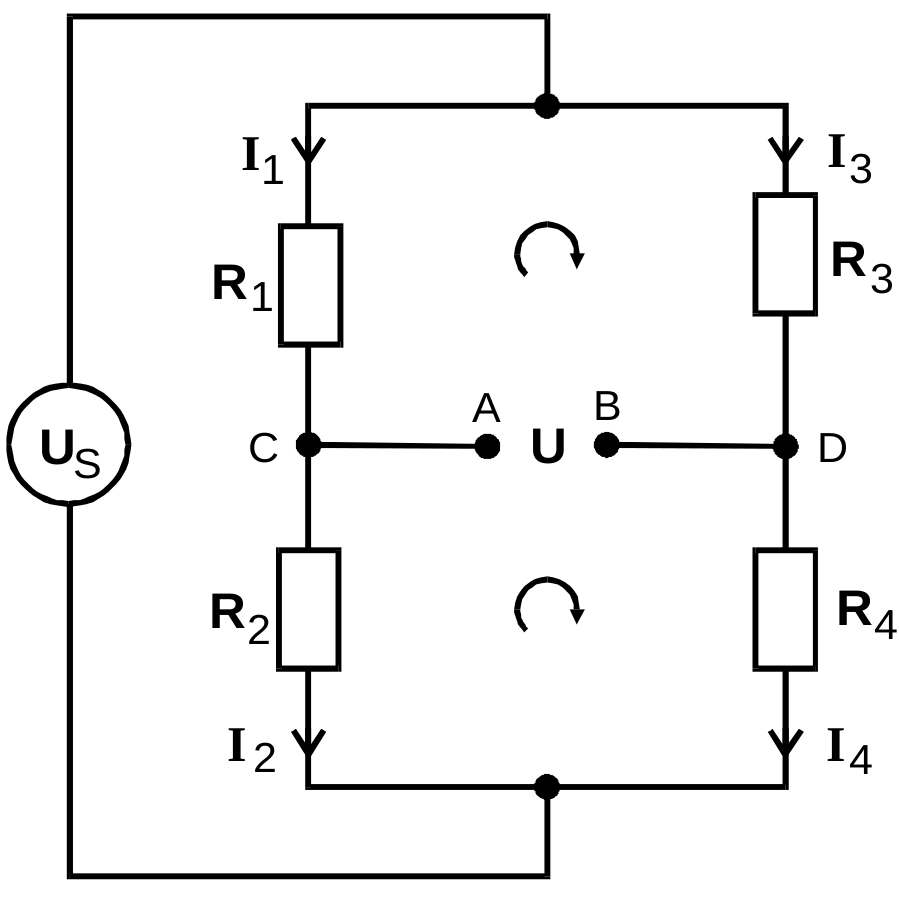
\includegraphics[width=0.4\textwidth]{Bilder/Brueckenschaltung.png}
  \caption{Brückenschaltung \cite{sample}.}
  \label{fig:Brueckenschaltung}
\end{figure}
\begin{equation}
  \sum \limits_{k} I_k= 0
  \label{eq:knotenregel}
\end{equation}
Aus der Maschenregel ergibt sich, dass die Summe aller Spannungen um eine Masche
$0$ ist. Daher gilt dies auch für die Produkte der Ströme und Widerstände nach
der Gleichung $U=RI$.
\begin{equation}
  \sum \limits_{k} U_k=  \sum \limits_{k} I_k R_k
  \label{eq:Maschenregel}
\end{equation}

Aus den beiden Maschen in der Abbildung \ref{fig:Brueckenschaltung}, die die Punkte
A, B, C und D enthalten, lässt sich mit den Kirchhoffschen Gesetzen
der Ausdruck
\begin{equation}
  U=-R_1 I_1 + R_3 I_3
\end{equation}
schreiben. Durch Umformungen folgt schließlich
\begin{equation}
  R_1 R_4 =R_2 R_3   .
  \label{eq:Widerstand}
\end{equation}
Komplexe Widerstände lassen sich mit den selben Gleichungen beschreiben.
Wiederstände von Kapazitäten, Induktivitäten und ohmschen Widerständen lassen sich
wie in den folgenden Gleichungen darstellen.
\begin{align}
&\hat{Z}_C = \frac{-i}{\omega}  &  \hat{Z}_L=i\omega L & & \hat{Z}_R = R &
\end{align}
So dass wiederum folgende Gleichung gilt.
\begin{equation}
\hat{Z}_1\hat{Z}_4=\hat{Z}_2\hat{Z}_3
\end{equation}
\section{Brückenschaltungen}
\subsection{Wheatstonesche Brücke}
\begin{figure}
  \centering
  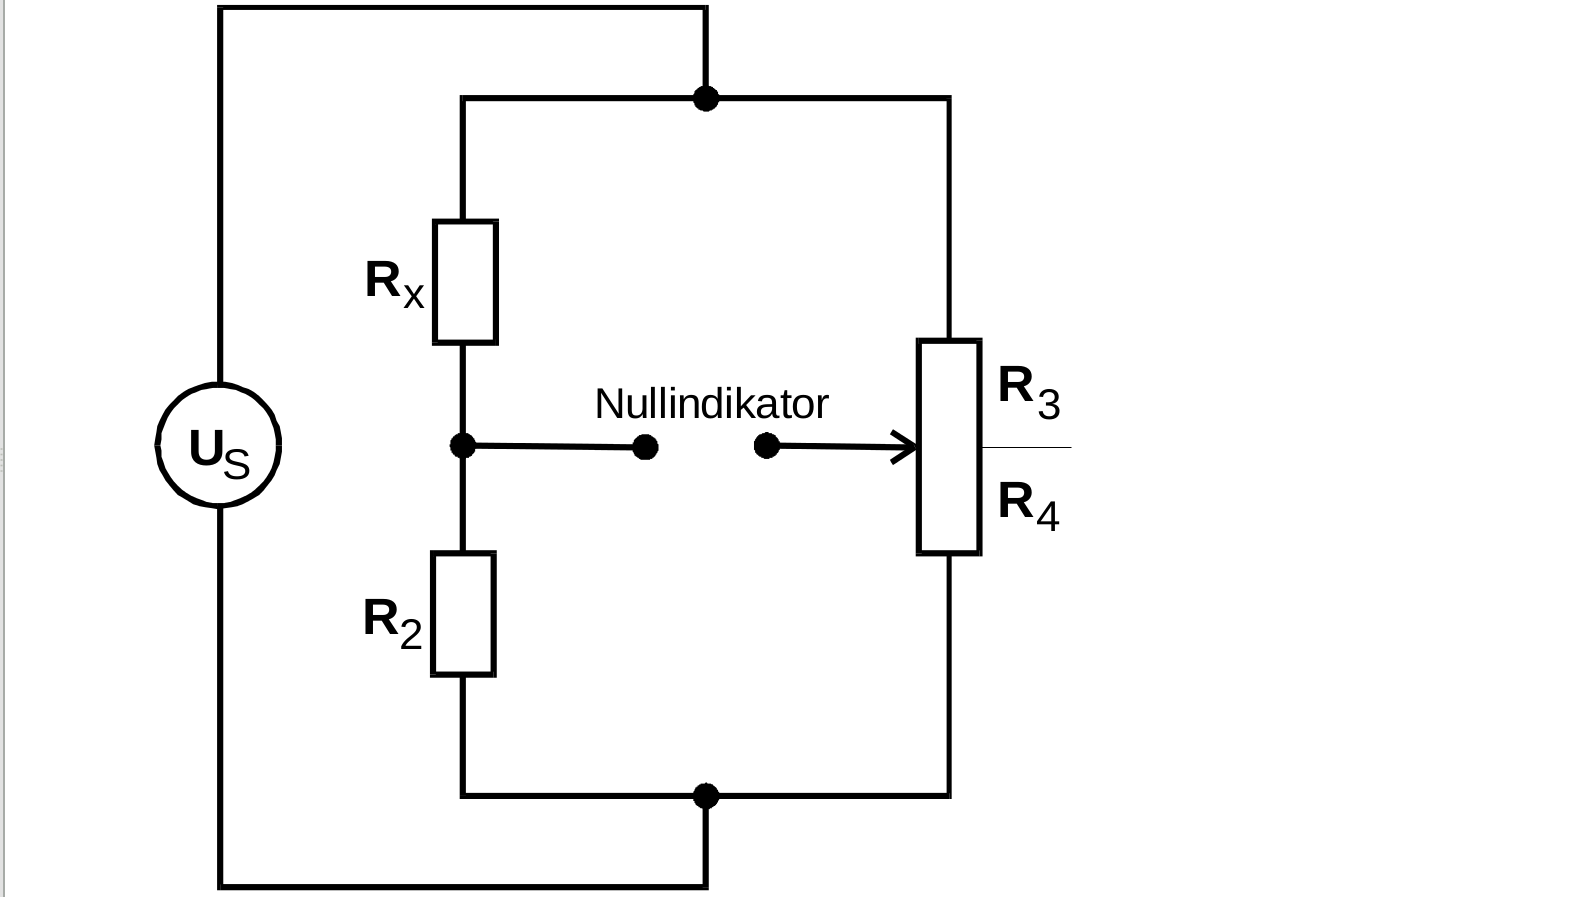
\includegraphics[width=0.4\textwidth]{Bilder/Wheatonsche.png}
  \caption{Wheatonsche Brückenschaltung\cite{sample}.}
  \label{fig:wheatonsche}
\end{figure}
Die Wheatstonesche Brückenschaltung kann mit Wechsel- und Gleichstrom betrieben werden,
da sie nur ohmsche Widerstände enthält. Die bekannten Widerstände $R_2$ $R_3$ und $R_4$
 müssen so variiert werden, dass die Potentialdifferenz verschwindet. Mit der
Gleichung\eqref{eq:Widerstand} ergibt sich der unbekannte Widerstand $R_\symup{x}$
aus\eqref{eq:Widerstand_Rx1}.
\begin{equation}
R_\symup{x}=R_2 \frac{R_3}{R_4}
\label{eq:Widerstand_Rx1}
\end{equation}
\subsection{Kapazitätsmessbrücke}
Werden die Widerstände $R_1$ und $R_2$ durch zwei Kapazitäten der Form
\begin{equation}
\hat{Z}_{C_{real}}=R-\frac{i}{\omega C}  ,
\end{equation}
ersetzt, ergibt sich eine Kapazitätsmessbrücke wie in Abbildung \ref{fig:capbruecke}.
Mit den Formeln \eqref{eq:Widerstand_Rx2} und \eqref{eq:Kapazitaet_Rx2} ergeben
sich die unbekannten Widerstände und Kapazitäten.
\begin{equation}
R_\symup{x}=R_2\frac{R_3}{R_4}
\label{eq:Widerstand_Rx2}
\end{equation}
\begin{equation}
C_\symup{x}=C_2\frac{R_4}{R_3}
\label{eq:Kapazitaet_Rx2}
\end{equation}
\begin{figure}
  \centering
  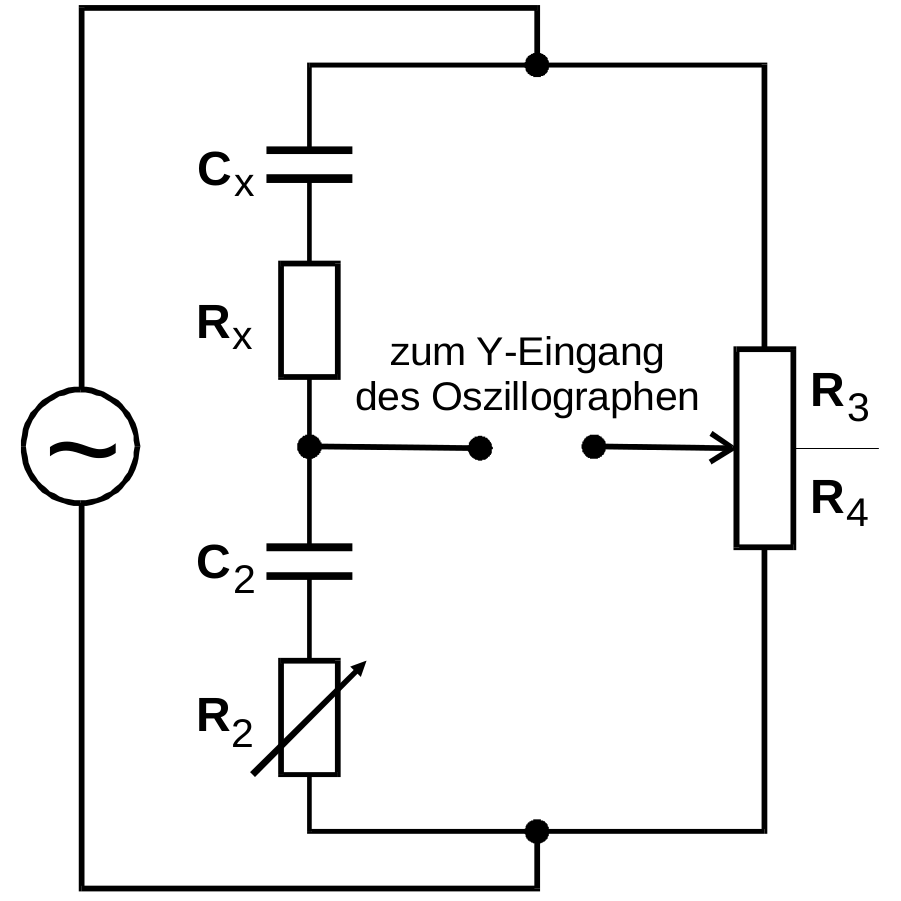
\includegraphics[width=0.4\textwidth]{Bilder/Capazitaetsbruecke.png}
  \caption{Kapazitätsbrücke\cite{sample}.}
  \label{fig:capbruecke}
\end{figure}
\subsection{Induktivitätenmessbrücke}
Werden die Kapazitäten und die dazugehörigen Widerstände durch Induktivitäten ausgetauscht,
 ergibt sich eine Induktivitätsmessbrücke wie in Abbildung \ref{fig:indbruecke}.
Mit den Formeln \ref{eq:Widerstand_Rx3} und \ref{eq:Induktivitaet_x2} lassen sich die
unbekannten Widerstände und Induktivitäten
\begin{equation}
R_\symup{x}=R_2\frac{R_3}{R_4}
\label{eq:Widerstand_Rx3}
\end{equation}
\begin{equation}
L_\symup{x}=L_2 \frac{R_3}{R_4}
\label{eq:Induktivitaet_x2}
\end{equation}
bestimmen.
\begin{figure}
  \centering
  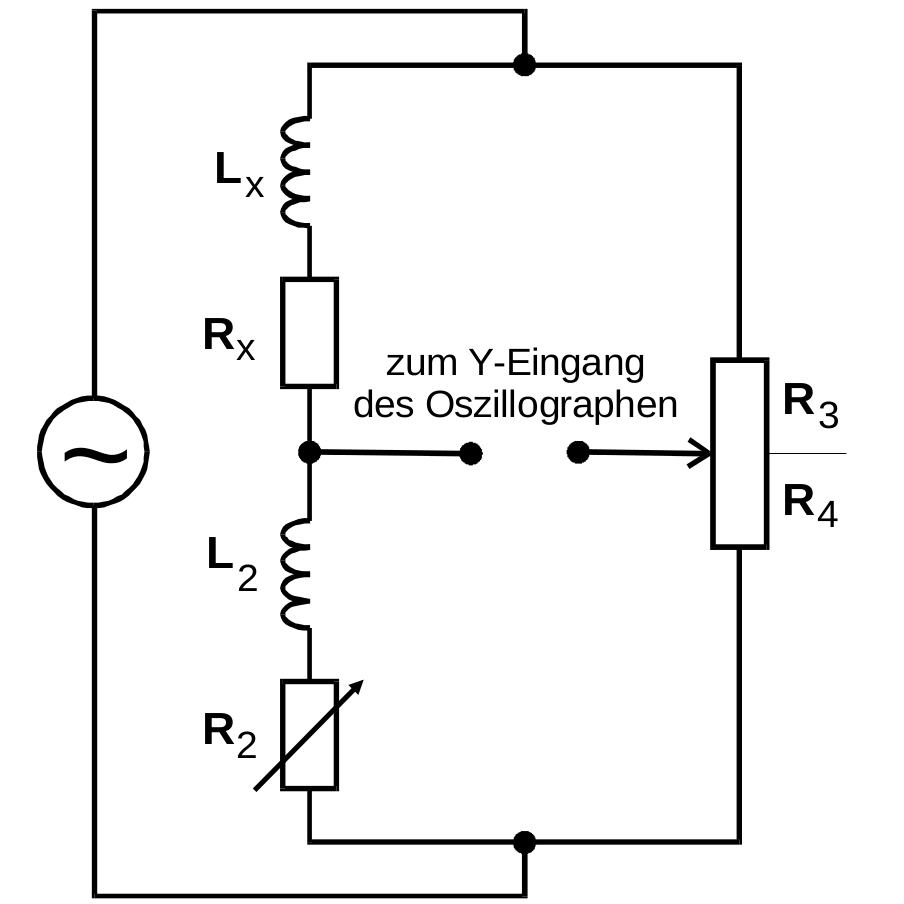
\includegraphics[width=0.4\textwidth]{Bilder/Induktivitaetsbruecke.png}
  \caption{Induktivitätsbrücke\cite{sample}.}
  \label{fig:indbruecke}
\end{figure}
\subsection{Maxwell-Brücke}
Mit einer Maxwellbrücke wie in Abbildung \ref{fig:Maxwellb} lassen sich mit
den Gleichungen \eqref{eq:Widerstand3} und \eqref{eq:Induktivitaet} unbekannte
Induktivitäten und Widerstände
\begin{equation}
R_\symup{x}= \frac{R_2 R_3}{R_4}
\label{eq:Widerstand3}
\end{equation}
\begin{equation}
L_\symup{x}=R_2 R_3 C_4
\label{eq:Induktivitaet}
\end{equation}
bestimmen. Im Gegensatz zur Induktivitätsmessbrücke
wird keine bekannte Induktivität benötigt.
\begin{figure}
  \centering
  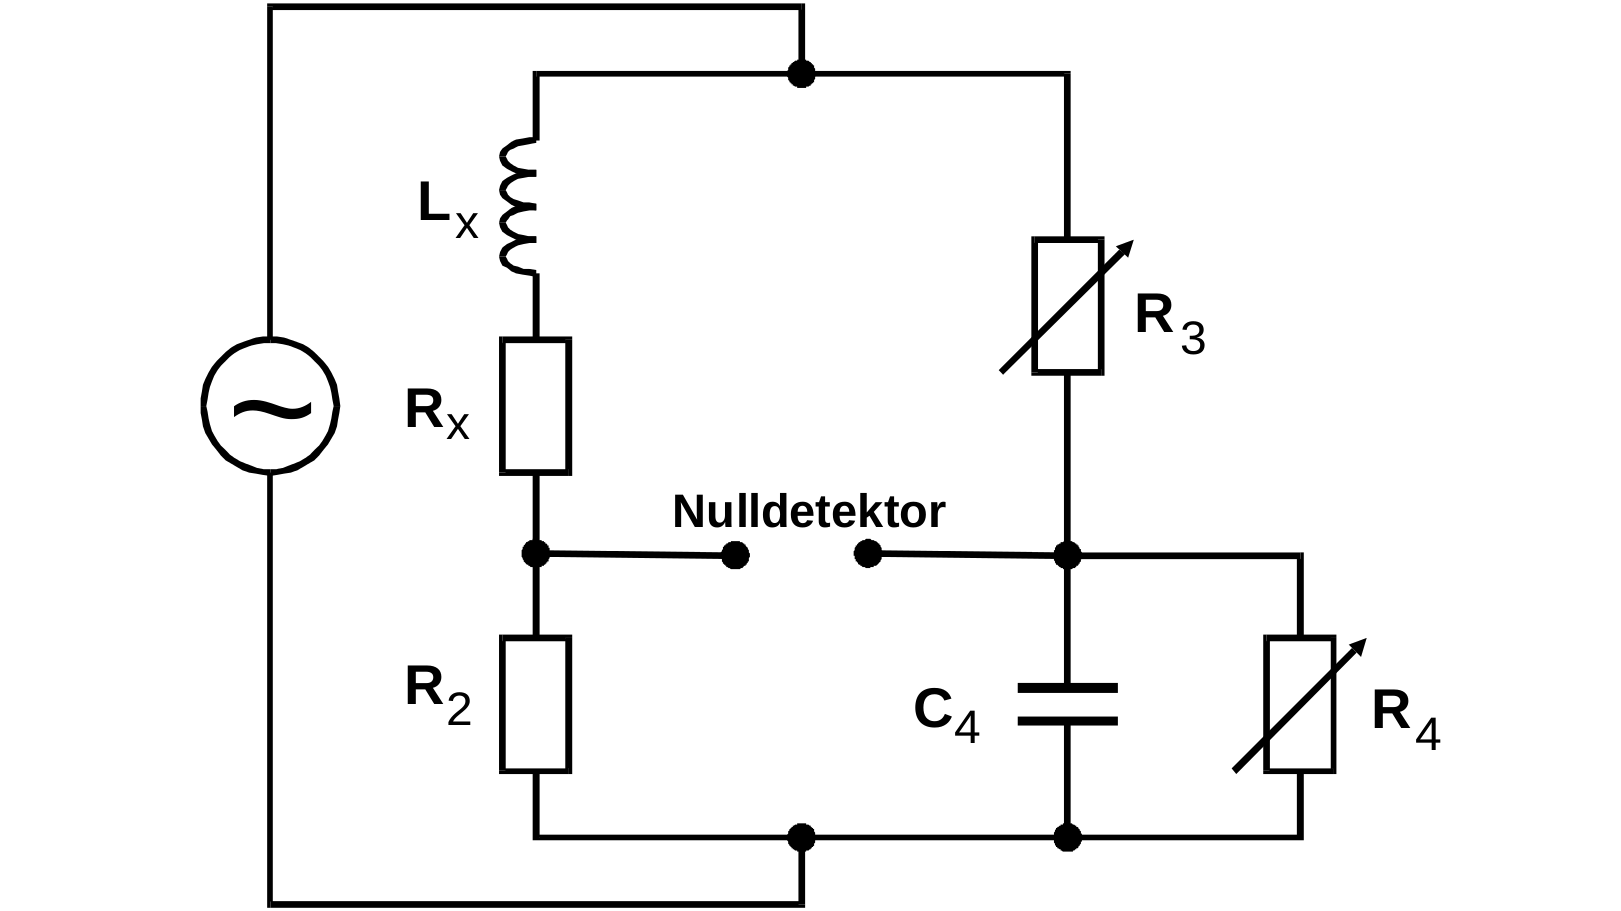
\includegraphics[width=0.7\textwidth]{Bilder/Maxwellbruecke.png}
  \caption{Maxwellbrücke\cite{sample}.}
  \label{fig:Maxwellb}
\end{figure}
\subsection{Wien-Robinson-Brücke}
\begin{figure}
  \centering
  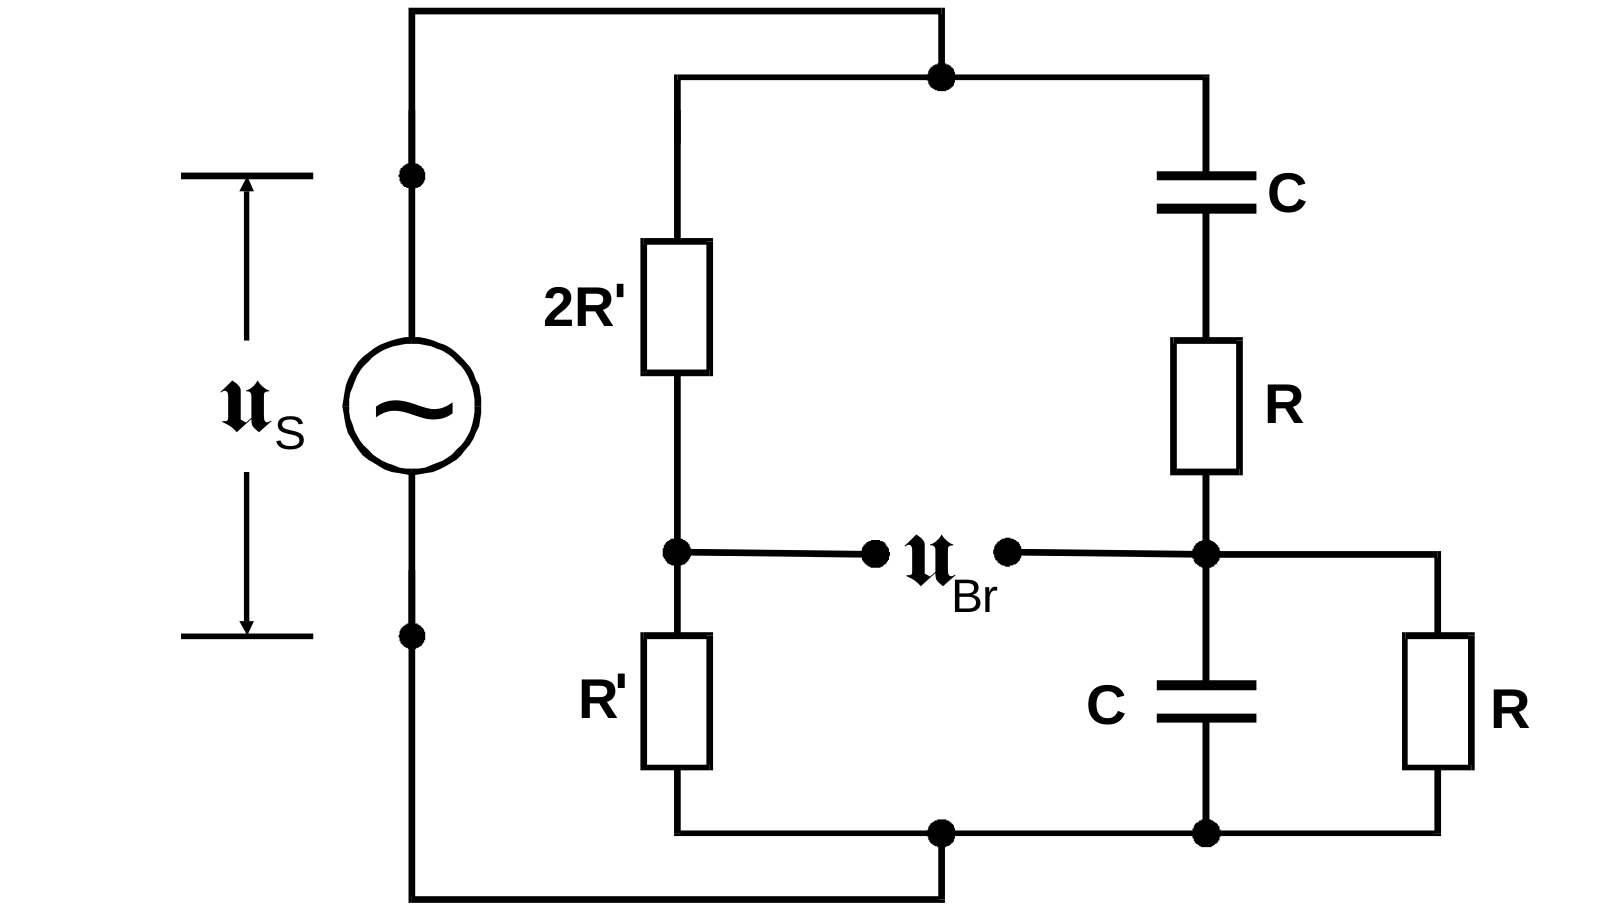
\includegraphics[width=0.7\textwidth]{Bilder/Wien_Robinsonbruecke.png}
  \caption{Wien-Robinson-Brücke\cite{sample}.}
  \label{fig:WBBruecke}
\end{figure}
Mit der Wien-Robinson-Brücke wie in Abbildung \ref{fig:WBBruecke} lassen sich
 bestimmte Frequenzen der Form
\begin{equation}
\omega_0=\frac{1}{RC}
\end{equation}
herausfiltert, da die Brückenspannung dann $0$ ist. Da die Bauteile $C,R$ und $R'$
sind alle bekannt, daher sollten sie eine möglichst geringe Toleranz haben und
die Kondensatoren einen möglichst geringen Verlust besitzen. Bei dieser
Brückenschaltung gilt die folgende Gleichung
\begin{equation}
  \left|\frac{U_{Br}}{U_S}\right|^2=\frac{(\omega^2R^2C^2-1)^2}
  {9\left((1-\omega^2 R^2 C^2)^2+9\omega^2R^2C^2\right)} \;.
  \label{eq:frequenz}
\end{equation}
An der Gleichung \eqref{eq:frequenz} ist zu erkennen, dass die Brückenspannung
für $\omega=\frac{1}{RC}$ verschwindet und ähnliche Frequenzen stark abschwächt.
Wird folgende Vereinfachung gewählt
\begin{equation}
\Omega:=\frac{\omega}{\omega_0}
\end{equation}
ergibt sich
\begin{equation}
  \left|\frac{U_{Br}}{U_S}\right|^2=\frac{1}{9}\frac{(\Omega^2-1)^2}
  {(1-\Omega^2)^2+9\Omega^2}  \; .
\end{equation}
Mit der Wien-Robinson-Brücke wird die Güte von Sinusspannungsgeneratoren gemessen.
Bei der Frequenz $\omega_0$ sollte die Brückenspannung verschwinden doch gibt es
keine perfekten Sinusspannungsgeneratoren wodurch nur ein Minimum entsteht das nicht
$0$ ist. Das Verhältnis der Oberwellen zur Grundwellen, die dies verursachen werden
im sogenannten Klirrfaktor ausgedrückt.
\begin{equation}
k:=\frac{\sqrt{\sum_{i=2}^N U_\symup{i}^2}}{U_1}
 \label{eqn:klirr}
\end{equation}
Die dafür benötigte Spannung $U_2$ wird mit der folgenden Formel berechnet.
\begin{equation}
U_2=\frac{U_{Br}}{f(2)}
 \label{eqn:U2berechnung}
\end{equation}
